\documentclass[11pt,a4paper]{book}

\usepackage[bottom=0.9in,top=0.85in,left=1in,right=1in]{geometry}
\usepackage{nopageno}
\usepackage{microtype}
\usepackage{parskip}
\usepackage[usenames,dvipsnames]{xcolor}
\usepackage{textcomp}    % textquotesingle
\usepackage{graphicx}
\usepackage{tcolorbox}   % fancy frame around a figure
\usepackage{siunitx}
\usepackage{booktabs}    % toprule, midrule, bottomrule
\usepackage{minted}      % code listings
\usepackage{tikz}        % tikz and fadings used in title page
\usetikzlibrary{fadings}

\setlength{\parskip}{\medskipamount}

\newcommand{\BookVersionString}{Version 0.1}
\newcommand{\BookVersionDate}{22 June 2021}

% ------------------------------------------------------------- Commands & Includes


% -------------- Problem number counter, chapter, question header

\newcounter{problemnumber}

\newcommand{\chaptermacro}[1]{\chapter*{#1}
  \addcontentsline{toc}{chapter}{#1}}

\newcommand{\questionheader}[1]{\stepcounter{problemnumber}
  \section*{\theproblemnumber\quad #1}
  \addcontentsline{toc}{section}{\theproblemnumber\hspace{0.5em} #1}}

\newcommand{\questionheadercontinued}[1]{{\Large\color{RoyalPurple}
  \theproblemnumber\quad #1\quad\textit{continued\dots}
  \vspace{18pt}
}}

% -------------- IN, OUT, colours, future reference, note

\newcommand{\IN}{\texttt{IN}}
\newcommand{\OUT}{\texttt{OUT}}

\definecolor{MyGrey}{gray}{0.45}
\newcommand{\grey}[1]{{\color{MyGrey}#1}}

\newcommand{\futurereference}[1]{\textbf{\color{Plum}Ref: #1}}
\newcommand{\note}[1]{\textbf{\color{Orchid}Note: #1}}

% -------------- Question, Input, Output, Sample, Explanation, ......

\newcommand{\Question}{\textbf{\color{purple}Question}\quad}
\newcommand{\Note}{\vspace{6pt}\textbf{\color{purple}Note}\quad}
\newcommand{\Input}{\vspace{6pt}\textbf{\color{purple}Input}\quad}
\newcommand{\Output}{\vspace{6pt}\textbf{\color{purple}Output}\quad}
\newcommand{\Sample}{\vspace{6pt}\textbf{\color{purple}Sample}\quad}
\newcommand{\Explanation}{\vspace{6pt}\textbf{\color{purple}Explanation}\quad}
\newcommand{\Scratch}{\vspace{6pt}\textbf{\color{purple}Scratch}\quad}
\newcommand{\Solution}{\vspace{6pt}\textbf{\color{purple}Solution}\quad}
\newcommand{\Notes}{\vspace{6pt}\textbf{\color{purple}Notes}\quad}
\newcommand{\Afterword}{\vspace{6pt}\textbf{\color{purple}Afterword}\quad}
\newcommand{\Running}{\vspace{6pt}\textbf{\color{purple}Running the code}\quad}
\newcommand{\Hint}{\vspace{6pt}\textbf{\color{purple}Hint}\quad}

% -------------- workedexample, stronghint

\newcommand{\workedexample}{{\color{purple}(worked example)}}
\newcommand{\stronghint}{{\color{purple}(strongly hinted)}}

% -------------- Python code listings

\newminted{python}{xleftmargin=2cm, linenos}
\newmintinline[pycode]{python}{}

% -------------- \sample and its encompassing minipagestwo and minipagesthree

%% % <hack> Frame all minipages, to aid in layout. Comment out when not wanted,
%% %        which is most of the time.
%% \let\minipagebak\minipage
%% \let\endminipagebak\endminipage
%% \newsavebox\TestBox
%% \renewenvironment{minipage}[2][]
%% {\begin{lrbox}{\TestBox}\begin{minipagebak}[#1]{#2}}
%% {\end{minipagebak}\end{lrbox}\fbox{\usebox{\TestBox}}}
%% % </hack>

\newcommand{\sample}[4]{%
  \begin{minipage}[t]{1.2cm}
    ~~~
  \end{minipage} %
  \begin{minipage}[t]{#1\textwidth}
    \textbf{IN}\\[3pt]
    \ttfamily
    #2
  \end{minipage} %
  \begin{minipage}[t]{#3\textwidth}
    \textbf{OUT}\\[3pt]
    \ttfamily
    #4
  \end{minipage}}

\newcommand{\minipagestwo}[2]{
  \begin{minipage}[t]{0.5\textwidth}
    #1
  \end{minipage} %
  \begin{minipage}[t]{0.5\textwidth}
    #2
  \end{minipage}}

\newcommand{\minipagesthree}[3]{
  \begin{minipage}[t]{0.33333\textwidth}
    #1
  \end{minipage} %
  \begin{minipage}[t]{0.33333\textwidth}
    #2
  \end{minipage} %
  \begin{minipage}[t]{0.33333\textwidth}
    #3
  \end{minipage}}

% -------------- environment for inline tables
%                  inlinetable  - bigkip above and below
%                  inlinetable* - medskip above, bigskip below

\newenvironment{inlinetable}{
  \bigskip
  \begin{center}
}{
  \end{center}
  \bigskip
}

\newenvironment{inlinetable*}{
  \medskip
  \begin{center}
}{
  \end{center}
  \bigskip
}



%\includeonly{
%  000-Titlepage,
%  000-Introduction,
%  100-overview,
%  100-who-is-the-tallest-1,
%  100-the-cheapest-tv,
%  100-shopping-1,
%  100-jogging-1,
%  100-who-is-the-tallest-2,
%  100-a-fair-wage-1,
%  300-overview
%}

% ==================================== Document ====================================

\begin{document}

% ----------------------------------------------- Title page, Contents, Introduction

\newgeometry{left=1in, right=1in,top=1in, bottom=0in}
{

\DeclareFixedFont{\titlefont}{T1}{ppl}{b}{}{0.5in}
\DeclareFixedFont{\subtitlefont}{T1}{ppl}{m}{it}{0.4in}
\DeclareFixedFont{\authorfont}{T1}{ppl}{sb}{}{0.3in}
\DeclareFixedFont{\versionfont}{T1}{ppl}{}{}{0.2in}
\DeclareFixedFont{\downloadfont}{T1}{ppl}{}{}{0.15in}

\definecolor{mytan}{HTML}{F6D5A8}
\pagecolor{mytan}

\colorlet{greytitle1}{black!95!}
\colorlet{greytitle2}{black!65!}
\colorlet{greytitle3}{black!75!}

\thispagestyle{empty}
\begin{flushright}
  \color{greytitle1}
  \titlefont High School Informatics\\[9pt] 
  \color{greytitle2}
  \subtitlefont for complete beginners\\[24pt]
  \color{greytitle3}
  \authorfont Gavin Sinclair
  \vfill
  \versionfont \BookVersionString \\[6pt] \BookVersionDate \\[12pt]
  \color{greytitle2}
  \downloadfont \BookDownloadText
  \vfill
\end{flushright}

\begin{center}
  \begin{tikzpicture}
    \node[scope fading=north, inner sep=0pt, outer sep=0pt]{
       \makebox[\textwidth]{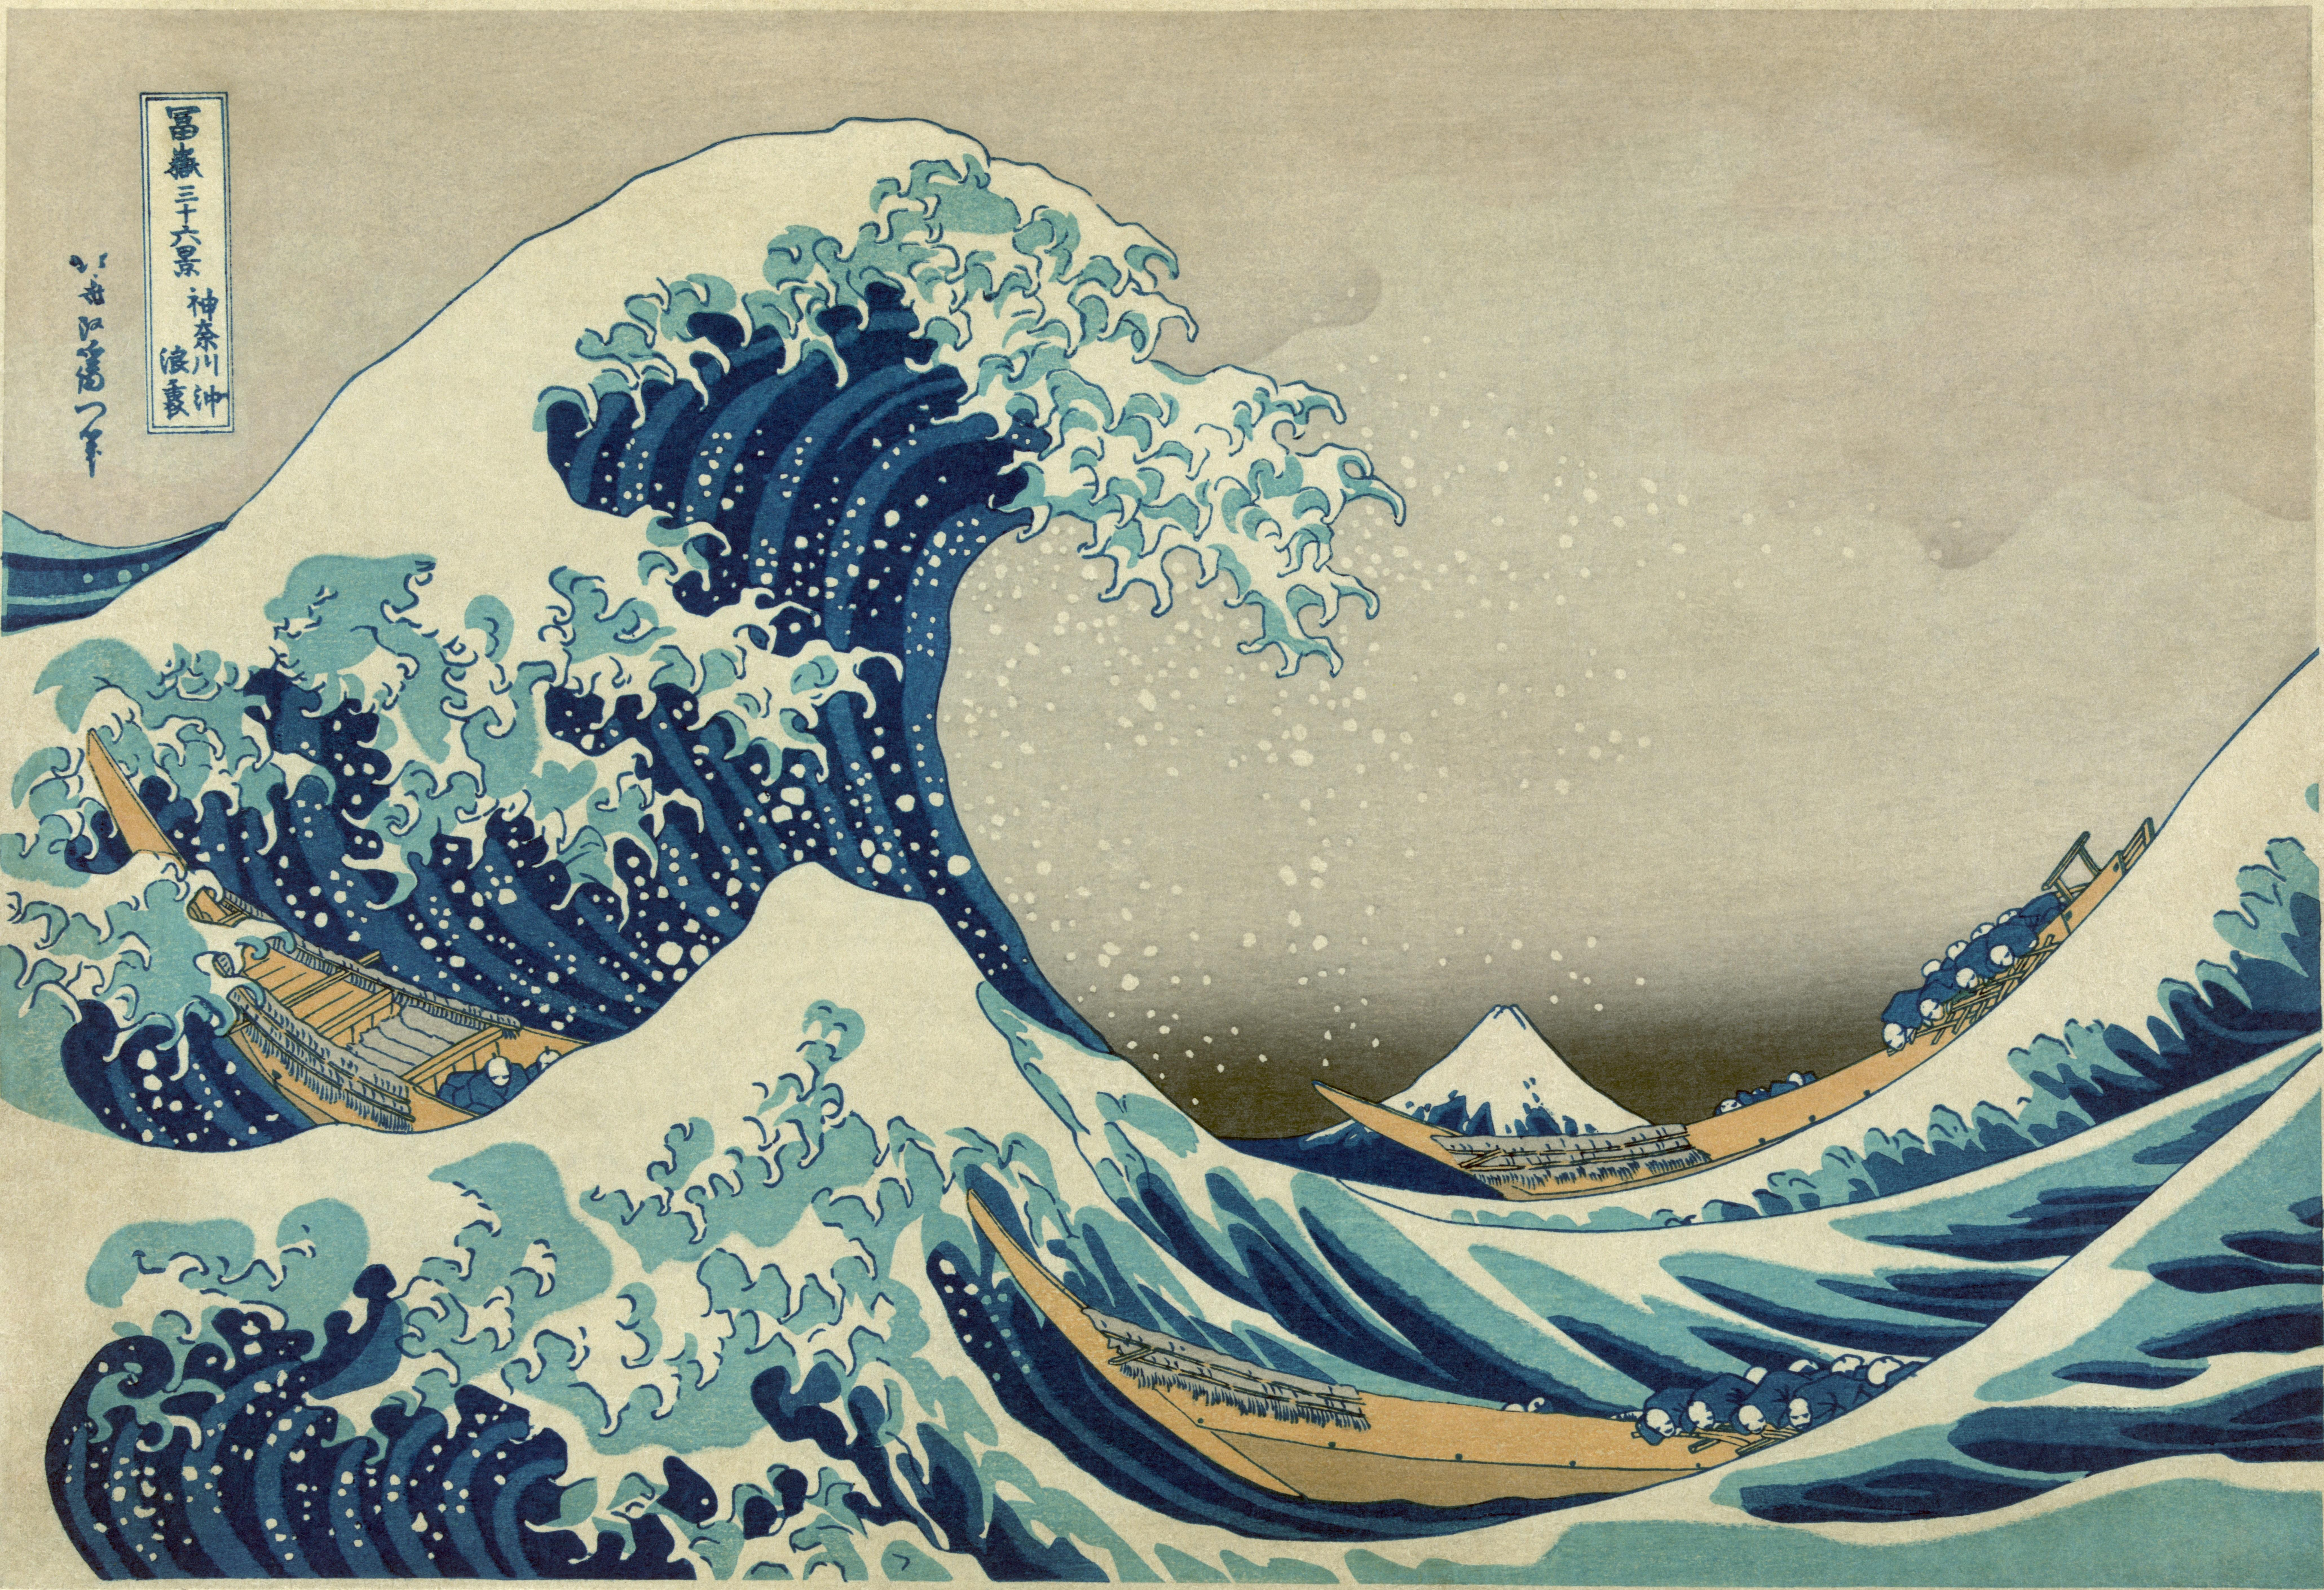
\includegraphics[width=\paperwidth]{images/kanagawa-wave.jpg}}
     };
   \end{tikzpicture}
 \end{center}

}


\clearpage

\restoregeometry
\nopagecolor

\tableofcontents


\chaptermacro{Introduction}

The exercises in this document will enable you to progress from absolute informatics
novice to a level of confidence sufficient to tackle elementary problems on
ORAC\footnote{ORAC is an online judge found at orac2.info. Many other online judges exist,
such as dmoj.ca, hackerrank.com, and so on. ORAC has excellent problems, but its
input/output system is a pain, especially for beginners, and its entry-level problems,
while very easy, are still too hard for complete beginners.}, such as \emph{Cute Numbers},
\emph{Ladybugs}, and \emph{Drought}.

These exercises are self-contained and do not involve submitting code to a website. You
do, however, need to set up your Python coding environment a little. This up-front
inconvenience pays off very quickly, though, as you can:
\begin{itemize}
  \item Solve all problems in one file.
  \item Run your code interactively, or test it against known data, or have it judged
    against secret data, all with ease.
\end{itemize}

\emph{Describe the PLC Informatics system, or refer to Appendix A or whatever...}

The problems in Series 100 are generally original, though some inspiration naturally comes
from easy problems I've seen before. They have only a modicum of context, unlike later
informatics problems that require you to read paragraphs of text to discern exactly what
the problem is. Some problems will even give you some or all of the code required to solve
them! The aim is for you to experience a minimum of friction in the early part of your
learning.

\emph{Idea: mention here that we want to get right into it, but if you are reading this
with some interest but wondering what it's actually all about, please see Appendix A
``What is informatics anyway?''}

For ease of navigating the document, problems appear one per page. Please turn over and
begin.

\section*{Problems to develop}
\begin{itemize}
  \item Input \texttt{940 5 . + 30 . -5 . + 100 . + 12 . - 4} representing a starting
    value and a series of additions and subtractions. Output \texttt{940 . 970 . 965 .
    1065 . 1077 . 1073} representing the starting value, the intermediate values, and the
    answer. Story can be something like profits and losses each week, and wanting to see
    that the business is afloat. Perhaps if an intermediate value is negative, the output
    can include a warning alongside it.
  \item Sarah has taken up jogging. She starts at $D$ metres per day and increases her
    distance by $I$ metres each day. How many days until she is running 10 kilometres per
    day?
  \item Siobhan has taken up jogging. She starts at $D$ metres per day and increases her
    distance by $I$ metres each day until she reaches her limit of $M$ metres per day.
    Find the total distance she covers in $N$ days.
  \item Find the length of a Collatz chain starting at a given number.
  \item Find which starting number between $A$ and $B$ produces the longest Collatz chain.
  \item Four people (Albert, Betty, Charlie, Dolly) play several games of Scrabble. They
    know who won each game but have lost track of their overall tally. Input: $N$ lines of
    names. Output: \texttt{Albert: 48 . Betty: 37} etc.
  \item Cute numbers
\end{itemize}


% ---------------------------------------------------------------- Chapter 1: Basics

\setcounter{problemnumber}{100}

\chapter{Operating on a fixed set of numbers}

In these problems, you will read in just one number, or a list of numbers of a known size.
You will calculate something or somethings based on the input and write it to output.

The example problems and solutions shown here demonstrate how to read numbers (integers
and floats) from \IN\ and write results to \OUT. Note that when we write a float%
\footnote{In computing, decimal numbers are generally called ``floats'', short for
    ``floating point numbers'', because the location of the decimal point can float around
    (consider 104.32 and 1.0432, for instance).}
to \OUT, we must round it to the specified number of decimal places to ensure predictable
output.%
\footnote{If you use Python, or pretty much any programming language, to calculate
  $0.1+0.2$ then you will get a surprising result. It's not Python's fault; we have to live
  with the fact that computers, by default, don't handle decimal numbers particularly
well.}

The following lines of code demonstrate how to input and output integers and floats. 

\begin{pythoncode} 
  import learninformatics as l

  def example1(IN, OUT):
    a = int(IN.readline())
    b = float(IN.readline())

    print("a squared:", a*a, file=OUT)
    print("b squared:", b*b, file=OUT)
    print("b squared (2dp):", round(b*b,2), file=OUT)
\end{pythoncode}

You should enter this code, then run it, then type \pycode|l.run(example1)| in your shell.
It will wait while you enter two numbers (an integer and a float) and will then
immediately output the squares that the code promises.

The first two problems in this chapter are complete worked examples to show input and
output in some more context and to demonstrate some decision-making. After that, problems
will have fewer hints as you are expected to apply the skills learned in the earlier
problems.

\begin{quote}
  \color{blue}
  To assist in your learning, you should have a notebook where you write out your solution
  to each problem, along with notes on what you have learned. You will find that you refer
  to it often.
\end{quote}

When you solve actual numbered problems, you will write functions with names like
\pycode|ex101| (short for ``exercise 101''. You can then run the function interactively,
as you did with \pycode|example1|, but you can also do something even better: run it
against test data and judging data. These ideas were explained in the Introduction.

% ---------------------------------------------------------------- 101 Classify a triangle

\clearpage

\questionheader{\theproblemnumber\ Classify a triangle \workedexample}

\Question Read three integers representing sides of a triangle and
determine whether the triangle is equilateral, isosceles, or scalene.

\Sample

\minipagesthree{\sample{0.25}{17\\14\\13}{0.25}{scalene}}
               {\sample{0.25}{13\\13\\8}{0.25}{isosceles}}
               {\sample{0.25}{5\\5\\5}{0.25}{equilateral}}

\Solution

\begin{pythoncode} 
  def ex101(IN, OUT):
    a = int(IN.readline())
    b = int(IN.readline())
    c = int(IN.readline())

    if a == b and a == c:
      answer = 'equilateral'
    elif a == b or a == c or b == c:
      answer = 'isosceles'
    else:
      answer = 'scalene'

    print(answer, file=OUT)
\end{pythoncode}

\Explanation\ Lines 2--4 read the three lines in \IN\ into integer variables $a$, $b$ and
$c$. Lines 6--11 determine the answer, and Line 13 writes the answer to \OUT.

This program is very much about making decisions (\pycode|if|/\pycode|elif|/\pycode|else|)
with a small amount of data. Note the use of \pycode|and| and \pycode|or| in making the
decisions. \pycode|elif| is short for ``else if''.

Line 1 wraps this code up in a function called \pycode|ex101|, which is what the
\textbf{learninformatics} environment expects to find when you...well, see below.

\Running

The Introduction explained the features of the \textbf{learninformatics} environment. Now
we see them for ourselves.

After you have \emph{Run} your code in replit.com, try the following in the console.
\begin{itemize}
  \item \pycode|l.run(101)|, then use the keyboard to enter the values \texttt{15},
    \texttt{15} and \texttt{13}. The answer \texttt{isosceles} should immediately be
    displayed.
  \item \pycode|l.run(101, "15\n19\n20\n")|. This puts the data in directly, instead of
    waiting for you to type it. The answer \texttt{scalene} should immediately be
    displayed.
  \item \pycode|l.samples(101)|. This runs your code against the three samples shown
    above and checks that the correct output is produced. If the output is incorrect, or
    if an error occurs, a helpful report is printed so you can try to work out what went
    wrong.
  \item \pycode|l.judge(101)|. This runs your code against a greater variety of inputs and
    checks for the correct output. The inputs remain secret, the information printed if
    something goes wrong is quite basic. If your code passes all tests, a success token is
    printed as a reward.
\end{itemize}

Note that the name of the function containing your solution is important. If you call it
\pycode|training101| or \pycode|unicorn|, or anything other than \pycode|ex101|, then the
actions above will not work.

\begin{tcolorbox}
  As you proceed through the exercises, you will have many \texttt{def}s in your code, one
  for each exercise. This is excellent: a record of your work that you can look back on.
\end{tcolorbox}


% -------------------------------------------------------------- 102 Calculate a gradient

\clearpage

\questionheader{\theproblemnumber\ Calculate a gradient \workedexample}

\Question Read four floats representing points $(x_1,y_1)$ and
$(x_2,y_2)$ and find the \emph{gradient} of the interval $AB$, which is typically called
$m$ and is calculated as follows:
\[ m = \frac{\mathrm{rise}}{\mathrm{run}} = \frac{y_2 - y_1}{x_2 - x_1}.\]

Output the gradient, rounded to three decimal places.  If the gradient is undefined
(because the run is zero), output \texttt{undefined}.

\Sample

\minipagesthree{\sample{0.25}{5\\1\\10\\3.5}{0.25}{2.500}}
               {\sample{0.25}{-2.76\\-1.01\\3.14159\\-10.559}{0.25}{-1.693}}
               {\sample{0.25}{3.7\\9.5\\3.7\\17}{0.25}{undefined}}

\Explanation\ The answers given reflect the following calculations:

\vspace{-5mm}
\minipagesthree{\[\frac{3.5-1}{10-5} = 2.5\]}
               {\[\frac{-10.559 - (-1.01)}{3.14159 - (-2.76)} = -1.692594\ldots\]}
               {\[\frac{17 - 9.5}{3.7 - 3.7} = \frac{7.5}{0}\]}


\Solution

\begin{pythoncode} 
  def ex102(IN, OUT):
    x1 = float(IN.readline())
    y1 = float(IN.readline())
    x2 = float(IN.readline())
    y2 = float(IN.readline())

    rise = y2 - y1
    run  = x2 - x1

    if run == 0.0:
      answer = 'undefined'
    else:
      answer = rise / run

    print(round(answer,3), file=OUT)
\end{pythoncode}

\Explanation\ Lines 2--5 read the four floats from \IN\ and assign them to sensible
variable names. Lines 7--8 calculate the rise and run, which are important values in
determining the gradient. Lines 10--13 determine the answer, looking out for the undefined
case. Line 15 outputs the answer to \OUT, rounding it to three decimal places as required.

\Running\ The function is named \pycode|ex102|, so you can:
\begin{itemize}
  \item Run the code interactively with \pycode|l.run(102)|.
  \item Test the correctness of the code against some data with \pycode|l.samples(102)|
    and \pycode|l.judge(102)|.
\end{itemize}

\questionheader{\theproblemnumber\ Who is the tallest (1)? \stronghint}

\Question\ In the schoolyard you determine who is the tallest by standing back to back.
Among your online friends, though, the only way to find this out is to compare numbers.
There are four people in your group, and so when everyone has entered their height in
centimetres, all that remains is to pick the largest number out of the list.

Your program will read four numbers from \IN\ and write the largest number to \OUT.

\Sample

\sample{0.2}{147\\165\\171\\168}
       {0.2}{171}

\Scratch\ We've seen several examples now of how to read an integer from \IN. For this
problem, we need to do it four times.

\begin{pythoncode}
    a = int(IN.readline())
    b = int(IN.readline())
    c = int(IN.readline())
    d = int(IN.readline())
\end{pythoncode}

We now have all our data. All that remains is to decide which is the largest of $a$, $b$,
$c$ and $d$.

\begin{pythoncode}
    if a >= b and a >= c and a >= d:
        ...
\end{pythoncode}

If the condition above is true, then $a$ is the largest of the four, or at least the equal
largest. What do we do in this scenario?

\begin{pythoncode}
    if a >= b and a >= c and a >= d:
        answer = a
\end{pythoncode}

We store the value of $a$ in a new variable called \emph{answer}.

To the two lines of code provided above, you can add six more to make a complete
determination of the largest value among $a$, $b$, $c$ and $d$.

\Solution\ A complete solution looks like this, except for the six lines you need to add.

\begin{pythoncode}
    def ex103(IN, OUT):
        a = int(IN.readline())
        b = int(IN.readline())
        c = int(IN.readline())
        d = int(IN.readline())

        if a >= b and a >= c and a >= d:
            answer = a
        #
        # ...six more lines...
        #

        print(answer, file=OUT)
\end{pythoncode}

If you're really stuck, you can look at the answers provided.

\Afterword\ The detailed assistance provided in this example was painstaking, so this will
be gradually decreased over the next few problems.

As you coded this problem, you might have had two questions.
\begin{itemize}
    \item Is this \emph{really} the best way to find the largest of four numbers?
    \item What if there were 400 numbers instead of four?
\end{itemize}

These questions will be addressed in \emph{Who is the tallest? (2)} and \emph{Who is the
tallest? (3)} respectively.


\questionheader{\theproblemnumber\ The cheapest TV}

\Question\ You walk the aisles of Bing Lee, looking for a new TV. You narrow it down to
five choices and decide to go with the cheapest. How much will you pay?

Your program will read five integers (representing prices in dollars) from \IN\ and write
the smallest number to \OUT.

\Sample

\sample{0.2}{499\\565\\325\\400\\717}
       {0.2}{325}

\Scratch\ If you have learned the lessons of the previous exercise well, you will complete
this one in no time. The running instructions are the same as before except the problem
name is \problemtagtt.

\Afterword\ Run your code as before. Brief instructions are included here for the last time:
\begin{itemize}
    \item \code{p.run(\problemtag)} to run it interactively using keyboard and screen.
    \item \code{p.test('\problemtag', \problemtag)} to run it against some test data and
      get detailed information if there is an error.
    \item \code{p.judge('\problemtag', \problemtag)} to run it against some judging data
      and get a token if you are successful.
\end{itemize}


\questionheader{\theproblemnumber\ Shopping (1)}

\Question\ You've just returned from the shops with the items you were asked to get. Your
dad asked ``How much was it?'', but you don't remember! You have to work it out quickly.
You bought exactly three \emph{kinds} of items, but different \emph{quantities} of each.

\Input

The input contains six lines: quantity 1, price 1, quantity 2, price 2, quantity 3, price
3. The quantities are integers in the range 1--10 and the prices are positive floats less
than 100 (representing \$100).

\Output\ The output is a single float containing the total price, and it must be rounded
to two decimal places.

\Sample

\sample{0.2}{6\\2.50\\8\\1.75\\3\\87.88}
       {0.2}{292.64}

\Explanation The output represents \$292.64, which is $6(\$2.50) + 8(\$1.75) + 3(\$87.88)$.

\Scratch\ You already know how to read an integer from \IN. See \futurereference{Appendix
...} for advice on reading and writing floats, especially outputing them rounded to two
decimal places.



\questionheader{\theproblemnumber\ Jogging (1)}

\Question\ Sarah is about to take up jogging. She will start jogging $D$ metres per day
and increase her daily distance by $I$ metres each day. When she reaches her target of $T$
metres per day, she will stop the daily increase and just keep a consistent jogging
pattern.

How many days after she starts will she reach her target?

\Input

The input contains three lines, all of which are values in metres:
\begin{itemize}
  \item $D$, the distance at which she starts jogging;
  \item $I$, the amount by which she increases her jog each day;
  \item $T$, her target daily jog, after which she doesn't increase it any further.
\end{itemize}

All values are integers, and you are guaranteed that $D < D+I < T$, that is, she will have
to apply at least two increases before reaching her target.

\Output\ You will write a single integer to \OUT, that being the number of days after
starting that she reaches her target.

\Sample

\minipagestwo{%
  \sample{0.4}{100\\50\\300}
         {0.4}{4} }{%
  \sample{0.4}{700\\20\\750}
         {0.4}{3} }


\Explanation In the first sample, her running pattern over the days goes like this:
\begin{center}
  \begin{tabular}{cc}
    Day & Distance (m) \\
    1   & 100\\
    2   & 150\\
    3   & 200\\
    4   & 250\\
    5   & 300
  \end{tabular}
\end{center}

She reaches her target on day 5, which is four days after she starts jogging, so the
answer is \texttt{4}.

In the second sample, her running pattern \emph{would} proceed 700, 720, 740, 760, but
\SI{760}{\m} actually exceeds her target of \SI{750}{\m}, so she would in fact run
\SI{750}{\m} on the fourth and subsequent days. In any case, she reached/exceeded her
target on day 4, which is three days after she started, so the answer is \texttt{3}.

\Scratch\ It is intended that you use simple mathematics to work this out. As a very large
hint, consider the expression $(300 - 100)/50$ in the first sample. As another hint, be
aware of the difference between \pycode|/| and \pycode|//| in Python. Finally, although
it's not strictly necessary, you might benefit from searching for examples of
\pycode|math.floor| and \pycode|math.ceil|.


\questionheader{\theproblemnumber\ Who is the tallest (2)?}

\emph{This question takes another look at \futurereference{Problem 101}.}

\Question\ In the schoolyard you determine who is the tallest by standing back to back.
Among your online friends, though, the only way to find this out is to compare numbers.
There are four people in your group, and so when everyone has entered their height in
centimetres, all that remains is to pick the largest number out of the list.

Your program will read four numbers from \IN\ and write the largest number to \OUT.

\Sample

\sample{0.2}{147\\165\\171\\168}{0.2}{171}

\Scratch\ Just like the earlier problem (\futurereference{Tallest person (1)}), we need to
read four integers from \IN. But this time, instead of making a lot of comparisons between
$a$, $b$, $c$ and $d$, we will use Python's built-in \code{max} function.

If you try the following Python expressions in your shell...

\begin{pythoncode}
    max(5, 1, 2, 9)
    max(7, 2, 5, 11, 6)
    max(-51, 73, 33, -1, 0, 12)
\end{pythoncode}

...then you will learn with some relief that Python has pretty much solved the ``Who is
the tallest?'' problem for us.

\Solution\ Make a new function \emph{in the same file}:

\begin{pythoncode}
    def train102(IN, OUT):
        a = int(IN.readline())
        b = int(IN.readline())
        c = int(IN.readline())
        d = int(IN.readline())

        answer = max(a, b, c, d)

        print(answer, file=OUT)
\end{pythoncode}

Use the tag \problemtagtt\ when you test and judge your code.

\Afterword\ The \pycode|max()| function can take any number of arguments, or it can find
the maximum of a (potentially very long) list. These are details for later. But here are
two teasers that you can run in the shell and think about.

\begin{pythoncode} 
  max(n*n for n in [-6, -4, -1, 0, 3])
  max(len(x) for x in ["Emma", "Caitlin", "Tim"])
\end{pythoncode}



\questionheader{\theproblemnumber\ A fair wage (1)}

\Question\ There are six employees in your company all doing roughly the same kind of
work. Some have worked for you for a longer time, or are generally more productive, so you
pay them a bit more. But once a year you take a look to see if the overall distribution of
wages seems to be fair.

The first thing you look for is the \emph{range} of wages: the highest minus the lowest.
You have a rule that the range should be less than 10\% of the highest wage.

\Input\ From \IN\ you will read six floats, each representing a weekly wage.

\Output\ To \OUT\ you will write three values:
\begin{itemize}
  \item The range, rounded to two decimal places
  \item The highest wage, rounded to two decimal places
  \item \texttt{yes} or \texttt{no} according to whether your wages are fair
\end{itemize}

\Sample

\minipagestwo{\sample{0.4}{535.00\\517.50\\580.00\\575.89\\553.60\\521.45}
                     {0.4}{62.5\\580.0\\no}}
             {\sample{0.4}{535.00\\517.50\\570.00\\570.00\\553.60\\521.45}
                     {0.4}{52.5\\570.0\\yes}}

\Explanation\ In the first sample, the range is about 10.78\% of the maximum wage, thus
the wages are not fair. In the second sample, the range is about 9.21\% of the maximum
wage, thus the wages are fair.

\Scratch\ After completing \emph{Who is the tallest? (2)}, you should be comfortable
reading six numbers and finding their maximum. To find the minimum, just use \pycode/min/
instead of \pycode/max/.

See the first code listing in Chapter 1 if you need a refresher on outputing floats
rounded to two decimal places.



% ---------------------------------------------------------------- Chapter 2: Loops (1)

\setcounter{problemnumber}{200}

\chapter{Looping through data}

In the problems you've encountered so far, you would:
\begin{itemize}
  \item read a fixed number of items from \IN;
  \item perform some calculation on those items;
  \item write a result to \OUT.
\end{itemize}

I'm sure you understand, though, that most problems don't come with a fixed number of
items of input, and sooner or later you will need to write code that can handle input of
any size. Well, that time is now.

\questionheader{\theproblemnumber\ Shopping (2)}

\Question\ You are in the middle of a sizeable shopping trip and realise you may not have
enough money to pay for everything you have put in your trolley. Quickly, you write a
program that takes in the quantities and prices of all the items you intend to purchase
and reports the total price.

\Input

The first line of input is $N$, which is the number of quantity-item pairs. Following this
are $2N$ lines, each pair of which contains the quantity and the price. The example will
make this clear.

\begin{itemize}
  \item $0 < N < 10\,000$.
  \item Each quantity $Q_i$ is an integer that satisfies $0 < Q_i < 1000$.
  \item Each price $P_i$ is a float that satisfies $0.00 < P_i < 1000.00$.
\end{itemize}

\Output\ The output is a single float containing the total price, and it must be rounded
to two decimal places.

\Sample

\sample{0.2}{5\\4\\2.99\\1\\3.15\\2\\14.95\\19\\0.14\\7\\7.10}
       {0.2}{97.37}

\Explanation The output represents \$97.37, which is $4(\$2.99) + 1(\$3.15) + 2(\$14.95)
+ 19(\$0.14) + 7(\$7.10)$.



\questionheader{Scrabble tally}

\Question\ Four friends---Albert, Betty, Charlie and Dotty---have played a lot of Scrabble
games over the years. The competition has been pretty close, but they've all kind of
forgotten who has won how many games. Luckily, when moving house recently, Dotty unearthed
a long list of the winners of all their games! By processing this list, you will be able
to give them a full tally.

\Input\ The first line of \IN\ contains $N$, the number of winners listed. Following this
are $N$ lines, each of which contains the name \texttt{Albert}, \texttt{Betty},
\texttt{Charlie} or \texttt{Dotty}, representing the winner of one game.

\Output\ \OUT\ contains four lines, reporting a tally as seen in the sample.

\Sample

\sample{0.25}{10\\Dotty\\Albert\\Albert\\Charlie\\Dotty\\Albert\\Dotty\\Dotty\\Dotty\\Charlie}
       {0.2}{Albert: 3\\Betty: 0\\Charlie: 2\\Dotty: 5}

\Scratch\ In this problem, you are reading \emph{strings} for the first time. ``String''
is the computer-science word for textual data, presumably because the characters are
``strung'' together. To read a string, we could simply call \pycode|IN.readline()|, with
no \pycode|int(...)| or \pycode|float(...)| wrapper because we certainly do not want
Python to attempt to convert our names to numbers.

There's a sting quite literally in the tail, though, because when we read a line of data
from \IN, the resulting string has a newline character at the end, and we don't really
want that.

\questionheader{Area calculator}

\Question\ As you pore over your Maths homework, you tire of the seemingly endless and
pointless area calculations you have to do. All the circles, semicircles, rectangles,
squares, parallelograms and triangles demand so much attention, and you only have so much
to give. But if you write a program to do the calculations for you, you'll get this
wretched work done and have time for a camomile tea while watching \emph{Rick \& Morty}
before bed.

\Input

The input contains any number of lines, which represent the shape names and the values
required to calculate them. For circles and semicircles you get one value: the radius. For
rectangles, parallelograms and triangles, you get base and (perpendicular) height. For
squares, you get the length of one side. The last line of input is simply \texttt{stop}.

Your input will contain ten area calculations or fewer.

\Output\ The output contains several lines, each of which is the result of an area
calculation, which must be a float rounded to three decimal places.

\Sample

\sample{0.25}{circle\\4.6\\triangle\\12\\5\\parallelogram\\19\\4.5\\
             square\\19\\rectangle\\7.2\\3.6\\stop}
       {0.2}{66.476\\30.0\\85.5\\361.0\\25.92}

\Scratch\ This problem differs from the earlier ones in two ways:
\begin{enumerate}
  \item We are \emph{not} told at the beginning how many lines there will be.
  \item Depending on the shape, we may need to read one line or two.
\end{enumerate}

Therefore, you deserve some help with this problem.

To solve \#1, we want to loop \emph{endlessly} and break out of the loop when we read
\texttt{stop}. This can be done with the following code structure:
\begin{pythoncode}
  while True:
    # ...
    if (condition):
      break
    # ...
\end{pythoncode}

The \pycode|while True| part creates the endless loop, and the \pycode|break| statement
gets out of it. Naturally, the \emph{condition} for us to break out is having read the
word \texttt{stop}.

Solving \#2 is not difficult and you probably don't need help with it, but just in case,
there is a hint on the next page.

\clearpage

\Hint

Here is the structure of the code, excluding the function header.

\begin{pythoncode}
  while True:
    shape = IN.readline().strip()
    if shape == 'stop':
      break
    elif shape == 'circle':
      radius = float(IN.readline())
      area   = 3.141592654 * radius * radius
      print(round(area,3), file=OUT)
    elif shape == 'rectangle':
      base   = float(IN.readline())
      height = float(IN.readline())
      # ...
    # etc.
\end{pythoncode}



\questionheader{Drought}

\Question\ \grey{(Sourced from ORAC)}\quad Years of drought have hit rural Australia hard.
With catchment levels at an all time low, you decide to purchase a rainwater tank. Soon
the winter rains arrive, and the tank slowly begins to fill.

You begin to wonder just when your tank will be entirely full. A friend
in the weather bureau has kindly lent you rainfall predictions for the next few days.
Given these predictions, and the size of your rainwater tank, write a program to determine
how many days your tank takes to fill.

\Input\ The first two lines of the input file will contain the values $N$ and $C$, where
$N$ is the number of days the weather predictions last, and $C$ is the capacity of your
rainwater tank in litres.  You are guaranteed that $1 \le N \le 1000$, and that $C$ is a
positive integer no greater than the total amount of rain that falls over the $N$ days.

The remaining $N$ lines of input will describe the rainfall levels for each day in order.
Each line will contain a single integer between 0 and 1\,000\,000: the amount of rain (in
litres) that will fall over your rainwater tank that day.

\Output\ Your output should consist of a single integer: the number of days until your
rainwater tank fills.

\Sample

\minipagestwo{%
  \sample{0.4}{6\\10\\2\\3\\3\\2\\2\\4}
         {0.4}{4} }{%
  \sample{0.4}{6\\11\\2\\3\\3\\2\\2\\4}
         {0.4}{5} }


\Explanation\ In both examples, the total rainfall changes as follows:

\begin{center}
\begin{tabular}{cc}
  \textbf{Day} & \textbf{Running total (L)} \\[3pt]
  1 & 2 \\[1pt]
  2 & 5 \\[1pt]
  3 & 8 \\[1pt]
  4 & 10 \\[1pt]
  5 & 12 \\[1pt]
  6 & 16 \\[1pt]
\end{tabular}
\end{center}
\vspace{12pt}

Hence a 10-litre water tank is full after 4 days and an 11-litre water tank is full after
5 days.

\Scratch\ If you intialise a variable to track the running total to zero at the beginning
and keep it updated as you read in the data, you should be able to solve this.

Good to know: you can \pycode|break| out of a \pycode|for| loop just like you can a
\pycode|while| loop.


\questionheader{Cute numbers}

\Question\ \grey{(Sourced from ORAC)}\quad For you, numbers have personalities. The number
4 is elegant, 18 is strong and 42 is enigmatic.  And, of course, any number ending in 0 is
cute.  The more zeroes at the end of a number, the cuter that number is. Therefore $70$,
$36\,640$ and $1\,800\,090$ are only a little bit cute (ending in just one zero), whereas
400 and $99\,200$ are very cute (ending in two zeroes) and $30\,000$ is really really cute
(ending in four zeros).

Your task is to read in a number $N$ and determine how many zeros are at the end of that
number, so you can tell just how cute the number is.

\Input\ The first line of input will consist of the single integer $d$, telling you how
many digits are in the number $N$. You are guaranteed that $1 \le d \le 100\,000$.

Following this will be $d$ additional lines, each containing a single digit (0, 1, 2, 3,
4, 5, 6, 7, 8 or 9). These will be the digits of $N$, written from left to right. You are
guaranteed that the first digit of $N$ will not be zero.

\Output\ You must write a single integer as output, representing the number of zeroes at
the end of $N$.

\Sample

\minipagestwo{%
  \sample{0.4}{5\\9\\9\\2\\0\\0}
         {0.4}{2} }{%
  \sample{0.4}{7\\1\\9\\0\\0\\0\\9\\0}
         {0.4}{1} }


\Explanation The first example describes $N = 99\,200$, which ends in two zeros. The second
example describes $N = 1\,800\,090$, which contains many zeroes within but has only one zero
at the end.


\include{200-high-wire-walk}

% ---------------------------------------------------------------- Chapter 3: Loops (2)

\setcounter{problemnumber}{300}

\chapter{Problems 3xx: operating on a list of numbers}

In these problems, ...



\questionheader{\theproblemnumber\ Jogging (2)}

\Question\ Sarah is about to take up jogging. She will start jogging $D$ metres per day
and increase her daily distance by $I$ metres each day. When she reaches her target of $T$
metres per day, she will stop the daily increase and just keep a consistent jogging
pattern.

Find the total distance she jogs in $N$ days.

\Input

The input contains four lines.
\begin{itemize}
  \item $D$, the distance (m) at which she starts jogging;
  \item $I$, the amount by which she increases her jog each day (m);
  \item $T$, her target daily jog (m), after which she doesn't increase it any further.
  \item $N$, the number of days for which we will calculate the total distance.
\end{itemize}

All values are integers, and you are guaranteed that $D < D+I < T$, that is, she will have
to apply at least two increases before reaching her target.

\Output\ You will write a single integer to \OUT: the total distance she jogs in $N$ days.

\Sample

\minipagestwo{%
  \sample{0.4}{100\\50\\2000\\6}
         {0.4}{1350} }{%
  \sample{0.4}{700\\20\\750\\6}
         {0.4}{4410} }


\Explanation In the first sample, over the first six days, Sarah runs a total of
$100+150+200+250+300+350=1350$ metres.

In the second sample, over the first six days, Sarah runs a total of
$700+720+740+750+750+750=4410$ metres.

\Scratch\ It is intended here that you sum the distances in a loop. It is possible to work
these out using mathematical formulas, but that is: (a) complicated; and (b) counter to
the spirit of this chapter.



% ---------------------------------------------------------------- Chapter 4: Lists

\setcounter{problemnumber}{400}


\chapter{Problems 4xx: miscellaneous problems}

There are no new skills in this chapter, just a range of problems for you to try.

There is one new thing to learn about reading input, however, and that is \textbf{reading
multiple inputs on the same line}. Problem 401 below demonstrates this.


% ---------------------------------------------------------------- Name, age, hourly rate

\questionheader{\theproblemnumber\ Name, age and hourly rate}

There is no ``question'' here, really. You will simply read data about multiple people
from three lines of \IN, and write that data to \OUT\ in a more readable format. In so
doing, you will learn how to read multiple values from one line, and how to use Python's
format strings.

\Sample

\sample{0.3}{James Lynne Toni Gerard\\
             23 21 20 21\\
             18.5 21.25 22.30 21}
       {0.6}{James is 23 years old and earns \$18.50 per hour\\
             Lynne is 21 years old and earns \$21.00 per hour\\
             Toni is 20 years old and earns \$22.30 per hour\\
             Gerard is 21 years old and earns \$21.00 per hour}

\Scratch\ To read multiple items from one line, we use Python's \pycode|split()| function.%
\footnote{Technically, \pycode|split()| is a \emph{method} of the \pycode|String| class.
That's more detail than we want at the moment. We'll think of it as a \emph{function} that
acts directly on string objects.}
If you try \pycode|"one two three four".split()| you'll get the idea of what
\pycode|split()| does.

So the four names in the sample can be read with:
\begin{pythoncode}
  names = IN.readline().split()
             # -> ['James', 'Lynne', 'Toni', 'Gerard']
\end{pythoncode}

The ages and hourly rates, however, need to be converted to integers and floats:
\begin{pythoncode}
  ages  = [int(x) for x in IN.readline().split()]
             # -> [23, 21, 20, 21]

  rates = [float(x) for x in IN.readline().split()]
             # -> [18.5, 21.25, 22.3, 21.0]
\end{pythoncode}

These are using Python's superpower, list comprehensions, which enable us to transform one
list---say, \pycode|['23', '21', '20', '21']|---into another, like \pycode|[23, 21, 20,
21]|.

You have two choices when it comes to understanding the above code:
\begin{enumerate}
  \item Memorise how to read multiple strings or ints or floats from one line, and leave
    it at that; or
  \item Understand fully how the code works so that you can use list comprehensions to
    power up your own code.
\end{enumerate}

The choice is yours, but you \emph{must} do at least \#1 above.

\Solution

\begin{pythoncode}
  def train401(IN, OUT):
    names = IN.readline().split()
    ages  = [int(x)   for x in IN.readline().split()]
    rates = [float(x) for x in IN.readline().split()]

    for i in range(len(names)):
      rate = round(rates[i],2)
      text = f'{names[i] is {ages[i]} years old and earns ${rate} per hour'
      print(text, file=OUT)
\end{pythoncode}

\Afterword Using another list comprehension, we can do all the float rounding in one go.
Here is a more sophisticated solution. Note Lines 5 and 8.

\begin{pythoncode}
  def train401(IN, OUT):
    names = IN.readline().split()
    ages  = [int(x)   for x in IN.readline().split()]
    rates = [float(x) for x in IN.readline().split()]
    rates = [round(x,2) for x in rates]

    for i in range(len(names)):
      text = f'{names[i] is {ages[i]} years old and earns ${rates[i]} per hour'
      print(text, file=OUT)
\end{pythoncode}

Also, we can push formatted strings further to create a nice tabular output. This will not
pass the test for problem \theproblemnumber, so it's named differently, but you can still
run it with \pycode|l.run(train401a)| and provide your own data.

\begin{pythoncode}
  def train401a(IN, OUT):
    names = IN.readline().split()
    ages  = [int(x)   for x in IN.readline().split()]
    rates = [float(x) for x in IN.readline().split()]
    rates = [round(x,2) for x in rates]

    print(f"{'Name:12} {'Age':>6} {'Rate:>7}", file=OUT)
    for i in range(len(names)):
      text = f'{names[i]:12} {ages[i]:>6} {rates[i]:>7}'
      print(text, file=OUT)
\end{pythoncode}


\include{400-shopping-3}

\questionheader{\theproblemnumber\ A fair wage (2)}

\Question\ In the years since you completed \emph{A fair wage (1)}, your company has
grown and grown, so the quaint idea of reading in just six numbers and assigning each to
its own variable to each has pretty much faded from memory. You now have $N$ workers and
want to do the same test: check that the \emph{range} of wages is no greater than 10\% of
the maximum wage. Except in recent times you've found the 10\% measure to be a little too
inflexible. So now the target percentage $P$ will be included in your data.

\Input\ From \IN\ you will read:
\begin{itemize}
  \item the integer $N$ ($5 < N < 1000$), the number of employees at your company;
  \item the float $P$ ($1.0 < P < 30.0$), the percentage used to determine whether the
    wages are fair;
  \item $N$ lines, each containing a float representing an employee's weekly wage.
\end{itemize}

\Output\ To \OUT\ you will write three values:
\begin{itemize}
  \item The range of wages, rounded to two decimal placs
  \item The highest wage, rounded to two decimal placs
  \item \texttt{yes} or \texttt{no} according to whether your wages are fair
\end{itemize}

\Sample

\sample{0.2}{7\\8.5\\635.17\\622.25\\631.02\\631.02\\628.56\\599.75\\608.10}
       {0.2}{35.42\\635.17\\yes}

\Explanation\ In the sample, the range is about 5.58\% of the maximum wage, which is less
than the target percentage 8.5\%, so the wages are fair.

\Scratch\ You know how to find the \pycode/max/ or \pycode/min/ of a group of individual
numbers, but in this problem you need the maximum and minimum of a \emph{list} of numbers.
That's no problem. The Python functions are very flexible:
\begin{pythoncode} 
  max(3,7,5,1,2)           # -> 7
  max([3,7,1,5,2])         # -> 7
\end{pythoncode}

There are five arguments in line 1 and only one argument (a list) in line 2, but the
result is the same. \pycode/max/ can take any number of arguments and knows what to
do if it is passed a single list.


\questionheader{Addition carry}

\note{This exercise assumes some experience with lists.}

\Question\ When two numbers are added, carry can be involved. Given two numbers, perform
the addition using the normal primary-school algorithm and output the number of times a
carry was performed.

Both numbers provided in \IN\ will be 1--20 digits long. They will not necessarily be the
same length.

\Sample

\begin{minipage}[t]{0.2\textwidth}
  \ttfamily
  \textbf{IN} \\
  19526\\
  32287
\end{minipage} %
\begin{minipage}[t]{0.2\textwidth}
  \ttfamily
  \textbf{OUT} \\
  3
\end{minipage}

\vspace{6pt}
\begin{minipage}[t]{0.2\textwidth}
  \ttfamily
  \textbf{IN} \\
  232\\
  51
\end{minipage} %
\begin{minipage}[t]{0.2\textwidth}
  \ttfamily
  \textbf{OUT} \\
  0
\end{minipage}

\Explanation\ The first example involves the following additions:
\begin{itemize}
  \item $6+7$ (generating a carry)
  \item $2+8+1$ (generating a carry)
  \item $5+2+1$
  \item $9+2$ (generating a carry)
  \item $1+3+1$
\end{itemize}

There are three carries.

The second example clearly involves no carries.

\Scratch\ To solve this problem we need to look at each number as a list of (numeric)
digits instead of a number \emph{per se}. So we read in the two numbers as strings and use
some special code that extracts the digits.

\begin{pythoncode}
  S1 = IN.readline()            # "19526"
  S2 = IN.readline()            # "2287"
  A = [int(x) for x in S1]      # [1, 9, 5, 2, 6]
  B = [int(x) for x in S2]      # [2, 2, 8, 7]
\end{pythoncode}

The code \pycode|for x in S1| iterates through each character \pycode|'1', '9', '5', '2',
'6'| in \pycode|S1|, and of course \pycode|int(x)| converts each of those to an integer.
Enclosing that code in \pycode|[...]| collects the generated values in a list. This kind
of code, called a \emph{list comprehension}, is a kind of superpower that Python has,
although it may be a bit daunting at first.

For the algorithm we are presently implementing, we would really like our two digit lists
to be in reverse order. The following code will do it.

\begin{pythoncode} 
  S1.reverse()                  # S1 is now [6, 2, 5, 9, 1]
  S2.reverse()                  # S2 is now [7, 8, 2, 2]
\end{pythoncode}

And now the digits line up and you can move \emph{forward} through the two reversed lists.

\Solution The rest of the code for this problem is an exercise for you.



% ---------------------------------------------------------------- Chapter 5 Mixed problems

\setcounter{problemnumber}{500}
\include{500-overview}

\questionheader{\theproblemnumber\ Golf (1)}

\Question\ Two people play a short game (nine holes) of golf, and you must write a program
to determine the winner.

Normally, the winner is the person with the lowest total score, where ``score'' means
``number of shots required to complete all holes''. But sometimes, players prefer to count
\emph{holes} instead of \emph{shots} to determine the winner. And this is one of those
times.

Say Jennifer won five holes, Kate won three holes, and one hole was tied. Then the result
would be \texttt{Jennifer won by 2 holes}. If Jennifer and Kate both won four holes and
one was tied, then we have to decide the winner by overall points, and the result might be
\texttt{Kate won by 3 points}. If both holes and points are tied, then the result is
\texttt{Jennifer and Kate tied}.

\Input\ From \IN\ you will read data from \emph{three lines}:
\begin{enumerate}
  \item The names of the two players
  \item The scores for the first player (nine integers)
  \item The scores for the second player (nine integers)
\end{enumerate}

\Output\ To \OUT\ you will write the result, as suggested by the paragraph above.

\Sample

\sample{0.3}{Jennifer Kate\\5 4 5 3 3 4 6 4 5\\4 4 5 4 4 4 5 4 4}
       {0.3}{Kate won by 1 hole}

\vspace{12pt}
\sample{0.3}{Jennifer Kate\\5 4 5 3 3 4 6 4 4\\4 4 5 4 4 4 5 4 4}
       {0.3}{Jennifer won by 2 points}

\vspace{12pt}
\sample{0.3}{Jennifer Kate\\5 4 5 3 3 4 6 4 4\\4 4 5 4 4 4 5 4 4}
       {0.3}{There was no winner}

\note{TODO: massage the data!}

\Explanation

\begin{itemize}
  \item In the first sample, Jennifer won two holes and Kate won three holes, so a winner
    can be determined by holes alone.
    \item In the second sample, Jennifer and Kate won three holes each, so points total
      points need to be considered. The points for Jennifer and Kate were 38 and 40
      respectively \note{TODO: check!}, and a lower score is better.
    \item In the third sample, Jennifer and Kate are equal on both holes and points.
\end{itemize}

\Scratch\ Ensure you've read the notes at the start of this chapter about reading multiple
values from one line.


% Several more problems to go here!

% ---------------------------------------------------------------- Chapter 6 2D data

\setcounter{problemnumber}{600}

\chapter{Two-dimensional data}

Intro text...

% ---------------------------------------------------------------- Cash grab (1)

\clearpage

\questionheader{\theproblemnumber\ Cash grab (1)}

Behind the gates of the walled city \emph{Adventis} lies an enormous $8 \times 10$ board
with 80 tiles, each one of them filled with coins. You are invited to choose which tile
to stand on and will be given one minute to scoop up as much cash as you can. Taking a
look from on high, you reason that wherever you stand, one minute will only afford you
enough time to get the cash on that tile and on all the immediately surrounding tiles.
That is, nine tiles in total.

On a scrap of paper, you jot down your estimate of how much cash is on each tile, and you
have only moments to decide where you will be placed.

\Input Eight rows of ten non-negative integers, each representing the cash amount on one
tile. The rows are numbered 1--8 and the columns 1--10, but these do not appear in the input.

For simplicity's sake, as this is your first exposure to two-dimensional data, all border
tiles will have a value of \texttt{0}.

\Output Two numbers \texttt{row col} identifying the most profitable place to stand.

\Sample

\sample{0.5}{0 0 0 0 0 0 0 0 0 0\\
             0 1 2 1 3 2 4 3 1 0\\
             0 4 1 2 1 3 0 2 0 0\\
             0 0 5 0 3 2 1 3 1 0\\
             0 2 7 8 5 4 2 0 3 0\\
             0 1 6 3 4 2 0 0 5 0\\
             0 3 0 2 2 1 2 2 3 0\\
             0 0 0 0 0 0 0 0 0 0}
       {0.2}{5 4}

\Explanation\ The location $(5,4)$ (in row-column notation) is the square with value
\texttt{8}, and the nine cells within reach are \texttt{5 0 3 7 8 5 6 3 4}, which clearly
produces a higher total than any other starting cell.%
\footnote{We can see the answer by eye in this case, but with different data it would not
be so easy.}

\Scratch\ We need to simulate standing in many different places and counting the
surrounding cash, and keep a running ``best location''. How many places do we need to try?
Well, the zeros on the outside mean there's no point standing on them. There's no point
standing \emph{next to} a row or column of zeros either, so that means we try all
locations in the rectangle $(2,2)$--$(8,8)$.

But first, we need to load the data in. We will create a list called \texttt{DATA} which
is really a list of \emph{rows}, each of which is a list of values. That is, when we're
done, we'll have (referring to the sample data):

\begin{pythoncode}
  DATA == [[0,0,0,0,0,0,0,0,0,0],    # Row 1 (index 0)
           [0,1,2,1,3,2,4,3,1,0],    # Row 2 (index 1)
           [0,4,1,2,1,3,0,2,0,0],    # Row 3 (index 2)
           # ...
           [0,0,0,0,0,0,0,0,0,0]]    # Row 10 (index 9)
\end{pythoncode}

Thus we have two-dimensional data as a list of lists. If we want to access the \texttt{4}
at row 2, column 7, then we use \pycode|DATA[1][6]|, noting zero-based indexing. Just
typing \pycode|DATA[2]| gives us the entirety of row 3.

Here is a way to get the values from \IN\ into our variable \pycode|DATA|.

\begin{pythoncode}
  DATA = []                # Start with an empty list and append each row.
  for i in range(8):
    row = [int(x) for x in IN.readline().split()]
    DATA.append(row)
\end{pythoncode}

Now to actually access all the data we want, from $(2,2)$ down to $(6,8)$, we can use a
loop within a loop. This is the normal way to deal with two-dimensional data.

\begin{pythoncode}
  for row in range(2,7):
    for col in range(2,9):
      print(f'Row {row+1}, Column {col+1}: {DATA[row][col]}')
\end{pythoncode}

It is worth trying this code to ensure you know what it does and why. Note that we are
translating between the 0-based indexing of lists and the 1-based language of the problem.

The double-loop above simulates standing in the 49 different locations from $(2,2)$ to
$(6,8)$. So what do we want to do in each location? We want to count all the cash in that
location and its eight neighbours.

\begin{pythoncode}
  for row in range(2,7):
    for col in range(2,9):
      cash = DATA[row-1][col-1] + DATA[row-1][col] + DATA[row-1][col+1] + \
             DATA[row]  [col-1] + DATA[row]  [col] + DATA[row]  [col+1] + \
             DATA[row+1][col-1] + DATA[row+1][col] + DATA[row+1][col+1]
\end{pythoncode}

With code like that, we might prefer to use \texttt{r} and \texttt{c} instead of
\texttt{row} and \texttt{col}. That will appear in the solution.

More than just count the cash, though, we need to see whether this is the best cash amount
we've encountered so far, and if so, remember where it is. For that we will use two
variables: \texttt{bestcash} and \texttt{location}. We will store the location as a
(row,column) pair.%
\footnote{Python conveniently allows us to store pairs or triples or ... of values in
round brackets. These are called \emph{tuples}, and once you've created them you can't
change them. You'll learn why not when you encounter the \emph{dictionary} data type.}

\Solution

\begin{pythoncode}
  def train501(IN, OUT):
    DATA = []
    for i in range(8):
      row = [int(x) for x in IN.readline().split()]
      DATA.append(row)
    
    bestcash = 0
    location = (0,0)

    for r in range(2,7):
      for c in range(2,9):
        cash = DATA[r-1][c-1] + DATA[r-1][c] + DATA[r-1][c+1] + \
               DATA[r]  [c-1] + DATA[r]  [c] + DATA[r]  [c+1] + \
               DATA[r+1][c-1] + DATA[r+1][c] + DATA[r+1][c+1]
        if cash > bestcash:
          # We have a new potential answer.
          bestcash = cash
          location = (r+1, c+1)

    row, column = location
    print(row, column, file=OUT)
\end{pythoncode}

\Explanation\ Much of the code was explained in \emph{Scratch} above. In Lines 7--8 we
initialise the two variables that help us find the best location, and in Lines 15--18 we
use them. In Line 18 we add 1 to the row and column because that is the numbering system
used in the problem. In Line 20 we \emph{unpack the tuple} into its two individual values
so that we can print them out with a space between. If we had called
\pycode|print(location)| then the output would be \texttt{(5,4)}.


% ---------------------------------------------------------------- Cash grab (2)

\clearpage

\questionheader{\theproblemnumber\ Cash grab (2)}

The question is the same as \emph{Cash grab (1)} but the board size is now variable. The
first line of \IN\ will contain the values $R$ and $C$, the number of rows and columns,
respectively. Following this will be $R$ lines, each containing $C$ non-negative integers.

\Sample

\sample{0.3}{...}
       {0.6}{...}

\Solution

\begin{pythoncode}
  def train501(IN, OUT):
    pass
\end{pythoncode}


% ---------------------------------------------------------------- Cash grab (3)

\clearpage

\questionheader{\theproblemnumber\ Cash grab (3)}

Variable size.

\Sample

\sample{0.3}{...}
       {0.6}{...}

\Solution

\begin{pythoncode}
  def train501(IN, OUT):
    pass
\end{pythoncode}


\include{600-golf-2}

% ---------------------------------------------------------------- END OF DOCUMENT

\vspace*{10cm}
\begin{center}
\textbf{End of document}
\end{center}

\end{document}
